\iffalse

\documentclass[12pt]{article}
\usepackage{graphicx}
\usepackage{amsmath}
\usepackage{mathtools}
\usepackage{gensymb}
\usepackage{amssymb}

\newcommand{\mydet}[1]{\ensuremath{\begin{vmatrix}#1\end{vmatrix}}}
\providecommand{\brak}[1]{\ensuremath{\left(#1\right)}}
\providecommand{\norm}[1]{\left\lVert#1\right\rVert}
\newcommand{\solution}{\noindent \textbf{Solution: }}
\newcommand{\myvec}[1]{\ensuremath{\begin{pmatrix}#1\end{pmatrix}}}
\let\vec\mathbf

\begin{document}
\begin{center}
\textbf\large{CLASS 11 CHAPTER-11 \\ LINES}

\end{center}
\section*{Excercise 10.2}


\solution
\fi
Let
\begin{align}
	\vec{A}&=x\vec{e_{1}},
	\vec{B}&=y\vec{e_{2}},
	\vec{P}&=\myvec{a\\b}
\end{align}
where
\begin{align}
	\vec{e_{1}}=\myvec{1\\0} \text{ and } \vec{e_{2}}=\myvec{0\\1}
\end{align}
as shown in Fig. \ref{fig:11/10/2/18Fig1}
\begin{figure}[!h]
	\begin{center} 
	    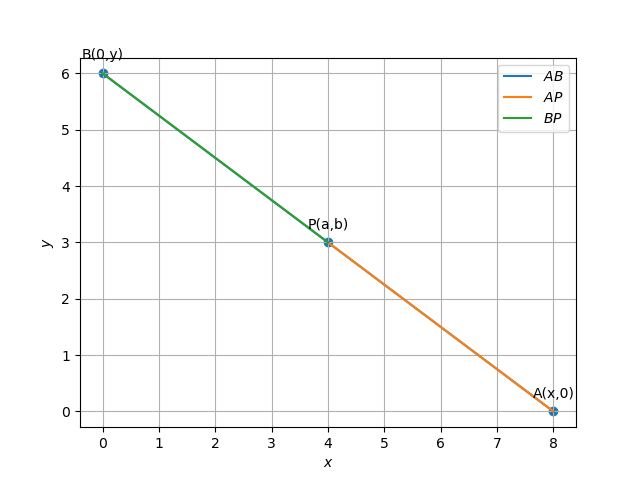
\includegraphics[width=\columnwidth]{chapters/11/10/2/18/figs/line1}
	\end{center}
\caption{}
\label{fig:11/10/2/18Fig1}
\end{figure}
Given that
\begin{align}
	\vec{P}&=\frac{\vec{A}+\vec{B}}{2}=\frac{x\vec{e_{1}}+y\vec{e_{2}}}{2}\\
\implies 	2\vec{P}&=x\vec{e_{1}}+y\vec{e_{2}}\\
	\vec{e_{1}}^{\top}\brak{2\vec{P}}&=\vec{e_{1}^{\top}}\brak{x\vec{e_{1}}+y\vec{e_{2}}}
=x\\				 
	\text{ and }\vec{e_{2}}^{\top}\brak{2\vec{P}}&=\vec{e_{2}^{\top}}\brak{x\vec{e_{1}}+y\vec{e_{2}}}
=y				 
\end{align}
Thus,
\begin{align}
	x&=2\vec{e_{1}}^{\top}\vec{P}=2a\\
	y&=2\vec{e_{2}}^{\top}\vec{P}=2b
\end{align}
yielding
\begin{align}
	\vec{A} &= 2a\vec{e_{1}}
	\vec{B} &= 2b\vec{e_{1}}
\end{align}
Thus, the direction vector of the line is 
\begin{align}
	\vec{m} &= \vec{A}-\vec{B}\\
	&=\myvec{a \\ -b}
\end{align}
and the normal vector is
\begin{align}
	\vec{n} = \myvec{b \\ a}
\end{align}
The equation of line passing through $\vec{P}$ is then obtained as
\begin{align}
	\vec{n}^{\top} \brak{\vec{x}-\vec{P}} &= 0\\
	\myvec{b & a}\vec{x} &= 2ab.
\end{align}


